%
% File acl2020.tex
%
%% Based on the style files for ACL 2020, which were
%% Based on the style files for ACL 2018, NAACL 2018/19, which were
%% Based on the style files for ACL-2015, with some improvements
%%  taken from the NAACL-2016 style
%% Based on the style files for ACL-2014, which were, in turn,
%% based on ACL-2013, ACL-2012, ACL-2011, ACL-2010, ACL-IJCNLP-2009,
%% EACL-2009, IJCNLP-2008...
%% Based on the style files for EACL 2006 by 
%%e.agirre@ehu.es or Sergi.Balari@uab.es
%% and that of ACL 08 by Joakim Nivre and Noah Smith

\documentclass[11pt,a4paper]{article}
\usepackage[hyperref]{acl2020}
\usepackage{times}
\usepackage{latexsym}
\usepackage[utf8]{inputenc}
\usepackage{amsmath} 
\usepackage{arabtex}
\renewcommand{\UrlFont}{\ttfamily\small}
\usepackage[utf8]{inputenc}
\usepackage{arabtex}
\usepackage{array}
\usepackage{booktabs} 
\usepackage{amssymb}  

\usepackage[hyperref]{acl2020}

\setlength{\parskip}{0pt}
\usepackage{times}
\usepackage{latexsym}
\usepackage{float}  
\usepackage{microtype}
\renewcommand{\UrlFont}{\ttfamily\small}
\usepackage{graphicx}  
\usepackage{booktabs}   
\usepackage{tabularx}  
\usepackage{array}      
\usepackage{pifont}    
\newcommand{\cmark}{\ding{51}} 
\newcommand{\xmark}{\ding{55}} 
\usepackage{tikz}
\usetikzlibrary{positioning, shadows, shapes, arrows.meta}
\usepackage{float} 
\usetikzlibrary{positioning, shadows} 




\usepackage{microtype}

\aclfinalcopy

%\setlength\titlebox{5cm}
% You can expand the titlebox if you need extra space
% to show all the authors. Please do not make the titlebox
% smaller than 5cm (the original size); we will check this
% in the camera-ready version and ask you to change it back.

\title{NLP701/805 Project 1
 \\ Evaluating Whisper’s Robustness for Medical Voice Command Understanding Using Text Classification with BERT }

\author{
 Ayah Al-Naji \\
  \texttt{ayah.al-naji@mbzuai.ac.ae} \\}
\date{}

\begin{document}

\maketitle
\begin{abstract}
This project examines the robustness of OpenAI's Whisper speech recognition model in deciphering surgical voice commands in various acoustic conditions. The aim is to assess how modifications like background noise, soft volume, speech rate, and frequency equalization impact the Accuracy of Whisper's transcription and the downstream text classification provided by BERT. I prepared a domain-specific database of 60 manually recorded medical spoken commands. To replicate an operating-room environment, I divided them into three categories (Request Instrument, Adjust Device, and Request Information). For Controllable augmentations, I used the Audacity software to make these different recordings. I added noise, reverb, bass, and treble effects, increasing the database to 120 samples. Whisper performed the best in clean speech (WER = 0.28, Accuracy = 63.3\%) and the worst in distorted audio (WER = 1.02, Accuracy = 6.9\%). Controllable augmentation helped increase robustness and yielded moderate downstream classification accuracy in BERT. These observations emphasize the role of acoustic diversity and illustrate the deficiency in the form of Whisper in adverse medical environments. In the future, I shall expand the study to the broader, more realistic MICCAI EndoVis database in order to compare the generalization performance in actual operating-room recordings.
\end{abstract}


\section{Introduction}

Voice-controlled systems in operating rooms are increasingly common, so hands-free communication can be established with robots and assistive devices. In high-stakes environments, accurate and robust speech recognition is crucial. Most commercial automatic speech recognition (ASR) systems, however, are initially learned under clean, general-purpose corpora and thus degrade or even crash when they come in contact with noise, speech overlap, or rapid command articulation. The limitation poses the biggest challenge in the practical application of ASR systems in real operating rooms.

This project involves the assessment of OpenAI's Whisper, a new state-of-the-art ASR model, in the medical voice command understanding scenario. The aim is to investigate how various acoustic distortions, i.e., background noise, speech speed variability, and equalization effects, impair Whisper's transcription accuracy and the resulting downstream classification loss of a command intent recogniser based on BERT.

I created a small domain-specific dataset of 60 manually recorded surgical commands across three categories: Request Instrument, Adjust Device, and Request Information. To simulate realistic operating-room conditions, I applied controlled augmentations using Audacity, including noise, reverb, bass, and treble effects, resulting in a total of 120 recordings. These variations allowed me to test Whisper's robustness under diverse acoustic conditions systematically.

Preliminary evaluations demonstrate that Whisper achieves good performance on clean speech yet has poor performance under distorted or low-audio-level command inputs. The loss in transcription quality also diminished the accuracy of the BERT classifier, highlighting the interdependence of ASR accuracy and downstream NLU. Future research will apply this study to a broader, in-vivo dataset—MICCAI EndoVis—to evaluate Whisper's generalization and robustness under practical surgical conditions.


\section{Related Work}
These previous developments in Automatic Speech Recognition (ASR) were motivated by end-to-end neural models like DeepSpeech \cite{hannun2014deepspeech} and Listen, Attend and Spell (LAS) \cite{chan2016las} that substituted the conventional pipelines with hybrid encoder–decoders. These models established that lots of labeled audio would result in competitive recognition performance. However, they provided no superior performance over previous systems in the scenario of noising or domain-transformation conditions.

To upgrade the robustness, \cite{ko2015audioaugment} proposed audio augmentation practices that were able to improve the overall generalization of ASR models, for instance, the combination of reverberation, background noises, and the inclusion of speed perturbation. The previously mentioned concept was later extended by SpecAugment \cite{park2019specaugment}, which made enormous performance achievements in large-scale tests by means of time-frequency domain masking across regions. In an attempt to improve real-world performance as well as noise robustness, Whisper \cite{pmlr-v202-radford23a} more recently benefited from extensive weak supervision as well as training over hundreds of thousands of multilingual and multitasking hours.

But, as \cite{alharbi2021asrreview} observe in the case of the present-day ASR systems, they too underperform in real situations, almost exclusively in the situations of invisible acoustics, technical vocab, or spontaneous human speech. Medical ASR, as pointed out by \cite{deepa2022speechhealthcare}, has to accommodate increased complexity in the healthcare scenario, in the form of domain expertise vocab, speech overlap, and high-stakes accuracy requirements, all of which, in turn, generate the requirements for the deployment of expert Data Collection and Adaptation Methods.

Unlike prior research, the present study centers around assessing Whisper's transcription robustness in controlled medical command situations and its downstream performance as tested when combined with BERT for intent classification. This practice, in turn, directly addresses how noising, reverb, and other practical effects impact both speech recognition and language comprehension—a dual-layer assessment much understudied in the prior literature. Table~\ref{tab:asr_comparison}compares previous research with the challenges in ASR tackled by this project, in which the new Whisper–BERT pipe has the strengths of previous research by paying close attention to robustness in the noisy clinical environment.

\begin{table}[h!]
\centering
\small
\begin{tabular}{l c c c c}
\hline
\textbf{Study} & \textbf{Noise} & \textbf{Aug.} & \textbf{Adapt.} & \textbf{Med.} \\
\hline
Hannun et al. (2014) & $\times$ & $\times$ & $\times$ & $\times$ \\
Chan et al. (2016) & $\checkmark$ & $\times$ & $\times$ & $\times$ \\
Ge et al. (2015) & $\checkmark$ & $\checkmark$ & $\times$ & $\times$ \\
Park et al. (2019) & $\checkmark$ & $\checkmark$ & $\times$ & $\times$ \\
Radford et al. (2023) & $\checkmark$ & $\checkmark$ & $\checkmark$ & $\checkmark$ \\
Alharth et al. (2021) & $\checkmark$ & $\times$ & $\checkmark$ & $\times$ \\
Deepa (2022) & $\times$ & $\times$ & $\checkmark$ & $\checkmark$ \\
mine & $\checkmark$ & $\checkmark$ & $\checkmark$ & $\checkmark$ \\
\hline
\end{tabular}
\caption{\small Comparison of ASR challenge coverage ($\checkmark$ = covered)}
\label{tab:asr_comparison}
\end{table}

\section{Proposed Method}
It presents a two-stage speech understanding pipeline that combines the state-of-the-art speech recognition model Whisper and the text classifier-based transformer BERT in order to identify and decode medical commands in the operating room environment. The architecture was tested under increasingly difficult acoustic conditions in order to investigate both transcription robustness and downstream classification robustness.


\subsection{Overview of the Pipeline}
The pipeline follows a sequential design composed of four key stages:

1. Automatic Speech Recognition (ASR) using Whisper.

2. Text-based Classification using BERT.

3. Audio Augmentation to assess noise and distortion robustness.

4. Merged Dataset Evaluation to simulate more realistic diversity.

Each step is based on the output of the previous step, as depicted in the Figure \ref{fig:pipeline}. Whisper converts the audio inputs into text, and the produced transcripts are then labeled by the BERT in one of the three command categories, i.e., Request Instrument, Adjust Device, or Request Information.


\subsection{Whisper Transcription Stage}

I executed the ASR stage by using the Whisper-small model.
60 manually annotated audio command sets were collected, with the sets being recorded in the following two ways:


1. Loud and clear


2. Rapid and silent, mimicking real-time situations in the operating room.

The transcriptions were produced automatically by Whisper, and the output was tested against a manually labeled ground truth, which I did. I used the Word Error Rate (WER) and Exact Sentence Accuracy results for evaluation, which showed that Whisper worked well for clean recordings (WER = 0.28, Accuracy = 63.3\%) but was poor for fast, low-level speech (WER = 1.02, Accuracy = 6.9\%).

\subsection{BERT Text Classification Stage}
I also fine-tuned a BERT-base-uncased classifier with the text-based transcriptions so that the classifier can cluster the commands in their respective semantic groups (Request Instrument, Adjust Device, and Request Information).

Because of the small size of the available dataset, I didn't reserve hard-coded test or dev splits. Instead, I used a 5-fold cross-validation strategy in order to obtain more robust and unbiased performance measures.

Here, the dataset was partitioned into five equal divisions (folds). In every round, four folds were applied for training purposes, while a single fold was used in evaluation, cycling through until all subsets had acted as the validation fold at least once. In that way, all the samples were featured in both training and testing in various runs. The total performance was then averaged over all the folds in order to reduce variance as well as overfitting effects, as shown in the diagram in Figure \ref{fig:crossval}, which shows in detail the cross-validation technique.
\begin{figure}[H]
\centering
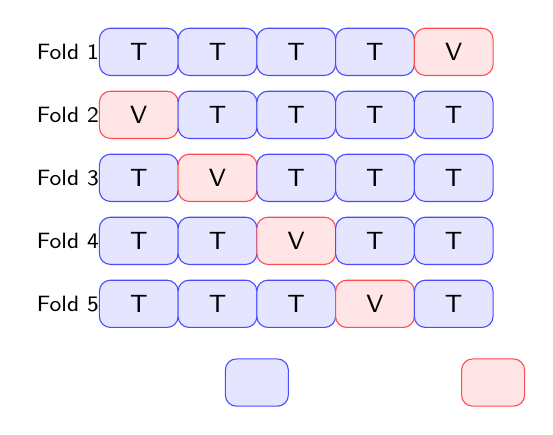
\begin{tikzpicture}[
  every node/.style={align=center, font=\sffamily\small},
  train/.style={rectangle, minimum width=1cm, minimum height=0.6cm, draw=blue!70, fill=blue!10, rounded corners},
  test/.style={rectangle, minimum width=1cm, minimum height=0.6cm, draw=red!70, fill=red!10, rounded corners},
  label/.style={font=\sffamily\footnotesize}
]

% Fold 1
\node[label, anchor=east] at (-0.3,0) {Fold 1:};
\node[train] (t11) at (0,0) {T};
\node[train] (t12) at (1,0) {T};
\node[train] (t13) at (2,0) {T};
\node[train] (t14) at (3,0) {T};
\node[test]  (t15) at (4,0) {V};

% Fold 2
\node[label, anchor=east] at (-0.3,-0.8) {Fold 2:};
\node[test]  (t21) at (0,-0.8) {V};
\node[train] (t22) at (1,-0.8) {T};
\node[train] (t23) at (2,-0.8) {T};
\node[train] (t24) at (3,-0.8) {T};
\node[train] (t25) at (4,-0.8) {T};

% Fold 3
\node[label, anchor=east] at (-0.3,-1.6) {Fold 3:};
\node[train] (t31) at (0,-1.6) {T};
\node[test]  (t32) at (1,-1.6) {V};
\node[train] (t33) at (2,-1.6) {T};
\node[train] (t34) at (3,-1.6) {T};
\node[train] (t35) at (4,-1.6) {T};

% Fold 4
\node[label, anchor=east] at (-0.3,-2.4) {Fold 4:};
\node[train] (t41) at (0,-2.4) {T};
\node[train] (t42) at (1,-2.4) {T};
\node[test]  (t43) at (2,-2.4) {V};
\node[train] (t44) at (3,-2.4) {T};
\node[train] (t45) at (4,-2.4) {T};

% Fold 5
\node[label, anchor=east] at (-0.3,-3.2) {Fold 5:};
\node[train] (t51) at (0,-3.2) {T};
\node[train] (t52) at (1,-3.2) {T};
\node[train] (t53) at (2,-3.2) {T};
\node[test]  (t54) at (3,-3.2) {V};
\node[train] (t55) at (4,-3.2) {T};

% Legend
\node[train, minimum width=0.8cm, label=right:{Training Set}] at (1.5,-4.2) {};
\node[test, minimum width=0.8cm, label=right:{Validation Set}] at (4.5,-4.2) {};

\end{tikzpicture}
\caption{Illustration of 5-fold cross-validation. Each fold uses 4 subsets for training (T) and 1 for validation (V). Metrics are averaged across all folds for robust evaluation.}
\label{fig:crossval}
\end{figure}

To obtain the final results, I averaged the performance metrics across all folds:


\begin{equation}
\bar{M} = \frac{1}{k} \sum_{i=1}^{k} M_i
\end{equation}

where $\bar{M}$ represents the averaged metric (e.g., accuracy, precision, recall, or F1-score), $M_i$ is the metric from the $i^{th}$ fold, and $k=5$ in this case.

BERT achieved a 5-fold average accuracy of 31.7\%, precision of 18.3\%, recall of 36.1\%, and F1-score.

\subsection{Audio Augmentation and Robustness Testing (Audacity)}
To examine the stability of Whisper against various forms of acoustic distortions, I used controlled audio augmentations with the software Audacity, a popular open-source audio manipulation software.
They mimic the actual-world operating room environments, like ambient noises, echo, and coloration of frequency.
I used two forms of augmentation:
(a) Noise Augmentation

I added white noise to account for the background noises of the operating room, such as the suction and ventilators. Table \ref{tab:noise_params} shows the specific parameters used for this augmentation. This approach helped me quantify how much Whisper's accuracy is compromised by acoustic interference in the sound signals.

Effect: White Noise

Tool: Audacity → Generate → Noise → White
\begin{table}[h]
\centering
\caption{White noise augmentation parameters}
\label{tab:noise_params}
Parameters for simulating operating room background noise.
{\small
\begin{tabular}{lll}
\hline
\textbf{Parameter} & \textbf{Value} & \textbf{Description} \\
\hline
Amplitude (0--1) & 0.02 & Loudness of added noise \\
Duration & Equal to original & Matches command duration \\
Mixing & Overlay & Keeps speech audible \\
\hline
\end{tabular}
}
\end{table}

(b) Reverb + Bass and Treble Adjustment


I applied Reverb and Bass/Treble Equalization to approximate OR acoustics and microphone variations. The parameters are in Tables~\ref{tab:reverb_params} and~\ref{tab:eq_params}. These tests assessed Whisper's robustness against Surgical environment distortions.
\begin{table}[h]
\centering
\caption{Reverb Parameters}
\label{tab:reverb_params}
{\small
\begin{tabular}{lll}
\hline
\textbf{Setting} & \textbf{Value} & \textbf{Description} \\
\hline
Room Size (\%) & 40 & Simulated reflection space \\
Pre-delay (ms) & 10 & Delay before first reflection \\
Reverberance (\%) & 50 & Controls reflection density \\
Damping (\%) & 50 & Controls decay rate \\
Tone Low (\%) & 100 & Maintains low frequencies \\
Tone High (\%) & 100 & Preserves high clarity \\
Wet Gain (dB) & +10 & Strength of reflected signal \\
Dry Gain (dB) & 0 & Keeps original loudness \\
Stereo Width (\%) & 100 & Preserves spatial width \\
\hline
\end{tabular}
}
\end{table}

\begin{table}[h]
\centering
\caption{Bass and Treble Parameters}
\label{tab:eq_params}
{\small
\begin{tabular}{lll}
\hline
\textbf{Setting} & \textbf{Value (dB)} & \textbf{Description} \\
\hline
Bass & +15 & Enhances low-frequency strength \\
Treble & +11 & Improves brightness and sharpness \\
Volume & +5 & Balances overall loudness \\
\hline
\end{tabular}
}
\end{table}

I re-evaluated Whisper on the augmented audio files after applying the modifications. The evaluation showed that the recording with noises added gave WER = 0.39 and Accuracy = 48.3\%, while the recording with reverb + bass \& treble gave WER = 0.57 and Accuracy = 35.7\%. It verifies the partial robustness of Whisper, indicating that light noise had a smaller effect while room reverberation and tonal coloration substantially distorted performance. Our experiments demonstrate the flexibility of Audacity for generating varied, natural-looking augmentations. Future researchers can extend their work by incorporating other effects, such as pitch shifting, time stretching, or compression, in order to better test Whisper and expand domain-specific training.

\subsection{Combined Dataset Training}
Once I produced all the augmented recordings, I combined all the subsets—original, noisy, and reverb-aided—into a 120-sample combined dataset. I used the combined dataset to refit the BERT classifier and study the effects of added acoustic diversity in text classification. The combined dataset reached an average 5-fold accuracy of 15.8\%, reflecting the challenge in coping with inconsistent transcriptions with augmentation types. However, there was an essential revelation in the step: the models that were exposed to acoustically diverse speech can generalize much better to the practical noise cases when fine-tuned correctly.

\section{Experiments and Evaluation Section}
I generated a 120-sample set of surgical voice directives, spread over three tasks: Request Instrument, Adjust Device, and Request Information. The recordings comprised the Normal and the Fast/Quiet conditions, which I amplified by white noise and reverb/equalization effects in the software, Audacity.

I transcribed all the audio samples using Whisper-small and then trained a BERT classifier on the resulting text for intent identification. I tested the pipeline in Google Colab Pro in accelerated mode with GPUs, with 5-fold cross-validation (batchsize = 8, learning rate = 2e-5) to evaluate both transcription accuracy and downstream classification accuracy.

\subsection{Whisper Evaluation and Results}
I evaluated the transcription result of Whisper by using Word Error Rate (WER) and Exact Sentence Accuracy (ESA). WER measures words that differ in the predicted and reference transcription, and ESA also monitors the number of accurately transcribed full sentences.
Together, these metrics measure both surface accuracy and semantic Accuracy. Whisper was tested under four recording conditions to evaluate robustness under various acoustic conditions. Its overall score was the highest on the loud, clean recording, while it plummeted on the fast and soft speech. Noise augmentation enhanced stability, while tonal change and reverb diminished recognition sharpness.

\begin{table}[h]
\centering
\caption{Whisper performance across recording conditions}
\label{tab:whisper_results}
\footnotesize
\begin{tabular}{lccc}
\toprule
\textbf{Recording Type} & \textbf{WER $\downarrow$} & \textbf{Acc. $\uparrow$} & \textbf{Interpretation} \\
\midrule
Normal (Loud) & 0.28 & 63.3\% & Best on clear, loud speech \\
Fast + Quiet & 1.02 & 6.9\% & Poor from unclear articulation \\
+ Noise & 0.39 & 48.3\% & Robust with background noise \\
+ Reverb + EQ & 0.57 & 35.7\% & Reverb reduced clarity \\
\bottomrule
\end{tabular}
\end{table}
\subsection{Whisper Performance Trend}
Whisper exhibited a sharp decline in Accuracy with rising distortion intensity, as can be seen in Figure~\ref{fig:accuracy_trend}. Noise offered modest gains, indicative of isolated robustness, while sophisticated reverb and changes in tone made the model's decoding of phonetics confuse.


\begin{figure}[h]
\centering
\includegraphics[width=0.9\linewidth]{Screenshot 2025-10-19 164738.png}
\caption{Whisper accuracy trend across distortion levels}
\label{fig:accuracy_trend}  % This line is essential
\end{figure}
\subsection{BERT Results and Discussion}
I trained a BERT intent classifier over three command categories based on the Whisper-generated transcriptions. I experimented with two training scenarios, one based solely on the initial set of 60 clean recordings, and the other based on the full set of 120 samples, incorporating augmented forms.

The BERT classifier performed relatively better when I trained it only on clean transcriptions, with an accuracy of 31.7\% and an F1-score of 23.2\%. The training set being extended to the inclusion of the noisy and the augmented set, however, made the performance drop in all the metrics, an accuracy of 15.8\% and an F1-score of 9.7\% being registered.

The unexpected finding is that while data augmentation in most cases fortifies model robustness, the noisy transcription under adverse acoustic conditions may have contributed to inconsistent patterns that the classifier was uncertain about. These conclusions lead us to believe Whisper's transcription consistency and quality matter more to downstream language understanding than the increase in the set size by way of acoustic variation.


\section{Conclusion and Future Work Section}
This study introduced an end-to-end pipeline for the decoding of spoken surgical commands by incorporating Whisper for transcription and intent classification based on BERT.
The experiment showed that Whisper holds steadily under the clean speech (WER = 0.28, Acc = 63.3\%) while the accuracy of the system decreases significantly under the noisy or reverberant conditions.
Therefore, the BERT averaged its clean transcription performance (Acc = 31.\%7) but reduced when it was fine-tuned over noisy, augmented data (Acc = 15.\%8), which supports the tight correlation of the quality of the ASR and downstream semantic interpretation.

In spite of this limitation, the experiments confirm the potential for creating lightweight command-understanding systems suited for surgical environments. It will involve the optimization of Whisper over medical data, studies of noising-robust architectures such as DistilBERT or transferable encoders, as well as the extension of the evaluation to the EndoVis MICCAI set for larger-scale and more realistic evaluation.






\bibliography{anthology,acl2020}
\bibliographystyle{acl_natbib}


\appendix


\section{Detailed Results Figures}

\begin{figure}[h!]
\centering
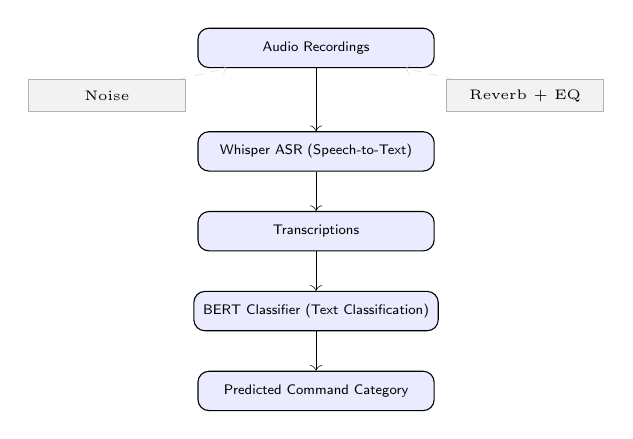
\begin{tikzpicture}[
  node distance=0.5cm,
  every node/.style={align=center, font=\sffamily\tiny},
  box/.style={rectangle, rounded corners, draw=black, fill=blue!8, minimum width=3cm, minimum height=0.5cm},
  small/.style={rectangle, draw=gray!60, fill=gray!10, minimum width=2cm, minimum height=0.4cm, font=\tiny}
]

% Vertical nodes
\node[box] (audio) {Audio Recordings};
\node[small, below left=0.2cm of audio] (noise) {Noise};
\node[small, below right=0.2cm of audio] (reverb) {Reverb + EQ};
\node[box, below=0.8cm of audio] (whisper) {Whisper ASR (Speech-to-Text)};
\node[box, below=0.5cm of whisper] (text) {Transcriptions};
\node[box, below=0.5cm of text] (bert) {BERT Classifier (Text Classification)};
\node[box, below=0.5cm of bert] (output) {Predicted Command Category};

% Vertical arrows
\draw[->, very thin] (audio) -- (whisper);
\draw[->, very thin] (whisper) -- (text);
\draw[->, very thin] (text) -- (bert);
\draw[->, very thin] (bert) -- (output);

% Augmentation arrows
\draw[->, dashed, gray!50, ultra thin] (noise) -- (audio);
\draw[->, dashed, gray!50, ultra thin] (reverb) -- (audio);

\end{tikzpicture}
\caption{Pipeline: Audio recordings are augmented with noise/reverb effects, transcribed by Whisper, and classified by BERT into medical commands.}
\label{fig:pipeline}
\end{figure}


\end{document}
